\chapter{Einleitung}
Hören die meisten Personen die Begriffe \enquote{Künstliche Intelligenz}
und \enquote{Maschinelles Lernen} stellen sie sich Roboter vor:
treue Diener, die all deine Aufgaben übernehmen oder eine tödliche Arme
von superintelligenten Cyborgs im Kampf gegen die Menschheit.
Künstliche Intelligenz (kurz KI) ist jedoch schon lange nicht mehr nur eine futuristische
Fantasie und Teil von Science-Fiction-Filmen; sie wird bereits großflächig
verwendet und findet Einsatz in einer Vielzahl von Anwendungen aus Bereichen
in nahe zu allen Teilen der Wirtschaft. Andrew Ng,
welcher unteranderem durch seine beliebten Onlinekurse zum Thema
Maschinellen Lernen (ML) und Deep Learning (DL)
bekannt ist,
\footnote{\url{https://www.coursera.org/instructor/andrewng}}
vergleicht KI mit der neuen Elektrizität.
\begin{aquote}{Andrew Ng \parencite{online:ai-andrew-ng}}
  \enquote{\textit{Just as electricity transformed almost everything 100 years ago,
      today I actually have a hard time thinking
      of an industry that I don’t think AI will
      transform in the next several years}}
\end{aquote}
Die Anwendung, mit der Maschinelles Lernen erstmalig öffentliche Aufmerksamkeit
erlangte und und noch immer das tägliche Leben vieler Menschen beeinflusst,
stammt aus den 90er-Jahren:
Die Rede ist von dem E-Mail-Spamfilter \parencite[1]{book:hands-on-ml}.
Es handelt sich um eine scheinbar einfache Aufgabe, welche
mit traditioneller Programmierung aber dennoch nur schwer gelöst werden kann.
Ein klassisches Programm besteht aus vielen statischen Regeln,
im Fall des Spamfilters können diese dazu dienen, auffällige Schlüsselwörter und
Satzteile zu erkennen (wie \enquote{Kreditkarte}, \enquote{konstenlos}, \enquote{kaufen} oder
andere Merkmale).
Ein statisches Programm ist nicht gut dafür geeignet, ein dynamisches Problem
zu beschreiben. Die Absender der Spamnachrichten könnten erkennen, welche E-Mails blockiert werden
und diese leicht abändern. Arbeiten sie so durchgehend um das Problem herum,
müssen immer wieder neue Regeln im Programm aufgenommen werden. Ein Spamfilter hingen,
welcher auf Maschinellen Lernen basiert, kann diese Regeln
selbstständig erkennen und automatisch anpassen wenn es eine Veränderung erkennt.
Der Algorithmus durchläuft hierfür eine Trainingsphase und verwendet dabei
Beispiel E-Mails (z.\,B. diese, die vom Benutzer markiert wurden)
und kann so lernen Spamnachrichten zu unterscheiden.
Diese Trainingsdaten werden als Trainingsdatensatz (engl. \textit{train set})
bezeichnet.
Es folgt ein Programm, welches weitaus kürzer,
einfacher zu verwalten und wahrscheinlich auch präziser ist.

\section{Was ist Maschinelles Lernen?}
Maschinelles Lernen ist die Wissenschaft (und Kunst) der Programmierung,
die es dem Computer ermöglicht, von Daten zu lernen. Arthur Samuel und Tom Mitchell
haben im Jahr 1959 und 1997 eine allgemeine und formale Definition gegeben \parencite[2]{book:hands-on-ml}:
\begin{aquote}{Arthur Samuel, 1959}
  \enquote{\textit{Machine Learning is the field of study that gives computers
      the abilty to learn without being explicitly programmed.}}
\end{aquote}
\begin{aquote}{Tom Mitchell, 1997}
  \enquote{\textit{A computer program is said to learn from experience
      $E$ with respect to some task \,$T$ and some performance measure $P$,
      if its performance on $T$, as measured by $P$, improves with experience $E$.}}
\end{aquote}
Betrachten wir erneut das Beispiel des Spamfilters, dann ist die Aufgabe $T$
das Markieren von Spam, die Erfahrung
$E$ sind die Trainingsdaten ist und der Bewertungsmaßstab $P$ bleibt zu definieren.
Es könnte zum Beispiel der Anteil der als richtig markierten E-Mails verwendet
werden. Dieser Maßstab heißt Genauigkeit und wird
häufig verwendet wenn es darum geht eine Klassifizierungsaufgabe zu bewerten.

\section{Die unterschiedlichen Lernmethoden}
Maschinelles Lernen kann genutzt werden, um eine Vielzahl von Problemen zu lösen.
Dies macht es zu einem mächtigen Werkzeug, aber auch eines, in dem es schwierig sein
kann, den Überblick zu behalten.
Da es viele verschiedene Systemen und Lösungsansätze gibt, ist es sinnvolle
diese in grobe Kategorien zu unterteilen.
Ein System kann unterschieden werden, basierend auf den folgenden
Kriterien \parencite[7]{book:hands-on-ml}:
\begin{itemize}
  \item Trainiert das System mit oder ohne menschlicher Betreuung, dann ist
        die Rede von überwachten und unüberwachten Lernen.
  \item Kann das System inkrementell mit einer Teilmenge der Trainingsdaten
        lernen oder verwendet es die gesamten Daten. Dieser Unterschied
        nennt sich \textit{online} vs. \textit{batch} Lernen.
  \item Funktioniert das System indem es lediglich neue Daten mit
        alten vergleicht oder kann es Muster erkennen, um beispielsweise
        einen Datensatz in Klassen zu unterteilen.
        Diese Lernmethoden nennen sich instanzbasiertes und modellbasiertes Lernen.
\end{itemize}
Keine der eben beschriebenen Kriterien schließen sich aus.
In einem echten System kann es sinnvoll sein, die verschiedenen
Eigenschaften zu kombinieren, um das gewünschte Ergebnis
zu erzielen. Der zuvor beschriebene E-Mail-Spamfilter
ist ein klassisches überwachtes und instanzbasiertes Lernsystem.
Es ist überwacht, da der Typ der E-Mail (z.\,B. durch Benutzereingabe)
bekannt ist und instanzbasiert da
der Algorithmus neue E-Mails mit alten vergleicht und das
Ergebnis so wählt, worin die größte Ähnlichkeit besteht.
Die Ergebnisse bei überwachten Lernen können wie im Falle des
Spamfilters vom Benutzer stammen oder durch Naturgesetzte und Expertenwissen
gegeben sein. Diese Daten werden im System als Label bezeichnet.
Wir können nun die einzelnen Lernmethoden etwas genauer untersuchen.

\subsection{Überwachtes Lernen}
Das bisherige Spamfilter Beispiel ist ein typisches
Klassifizierungsproblem. Zu einer Menge von eine Eingabewerten
(auch genannt Features) soll die Wahrscheinlichkeit bestimmt werden,
dass diese Feature zu einer bestimmten Klasse gehören.
Was ist aber wenn keine Wahrscheinlichkeiten
prognostiziert werden sollen, sondern numerische Werte wie
der Preis eines Autos? Dieses Problem nennt sich Regression.
Ein Beispiel soll zeigen wie das Prinzip funktioniert.
Es soll ein einfaches Modell trainiert werden welches eine lineare
Funktion modelliert. Als ersten Schritt müssen die Trainingsdaten generiert werden,
der folgende Python Code zeigt diesen Vorgang mithilfe von NumPy:
\begin{lstlisting}
import numpy as np
rng = np.random.default_rng(42)
x = 6 * rng.random((100, 1))
y = 5 + 3 * x
\end{lstlisting}
NumPy ist eine Python Bibliothek, welche das effiziente Rechnen mit
multidimensionalen Daten ermöglicht, zum Beispiel der Vektor- und Matrixmultiplikation.
\footnote{\url{https://numpy.org/doc/stable/user/whatisnumpy.html\#what-is-numpy}}
Operationen in NumPy werden immer elementweise durchgeführt, der folgende Programmausschnitt
zeigt dieses Verhalten:
\begin{lstlisting}
>>> a = np.array([1, 2, 3])
>>> a
array([1, 2, 3])
>>> a * 3
array([3, 6, 9])
\end{lstlisting}
CPUs und GPUs sind sehr gut darin diese Art der Berechungen durchzuführen,
was NumPy sehr viel schneller macht als die Verwendung einer expliziten Schleife.
Wir können nun die eben generierten Daten anzeigen und verwenden hierfür
eine weitere Python Bibliothek mit dem Namen Matplotlib:
\footnote{\url{https://matplotlib.org/stable/index.html}}
\begin{lstlisting}
import matplotlib.pyplot as plt
plt.plot(x, y, "b.")
plt.xlabel("$x_1$")
plt.ylabel(r"$5 + 3x$")
plt.axis([0, 6, 5, 25])
plt.show()
\end{lstlisting}
Die hieraus resultierende Grafik ist in \autoref{plot:linear-data} zu sehen.
\newpage
\begin{figure}
  \centering
  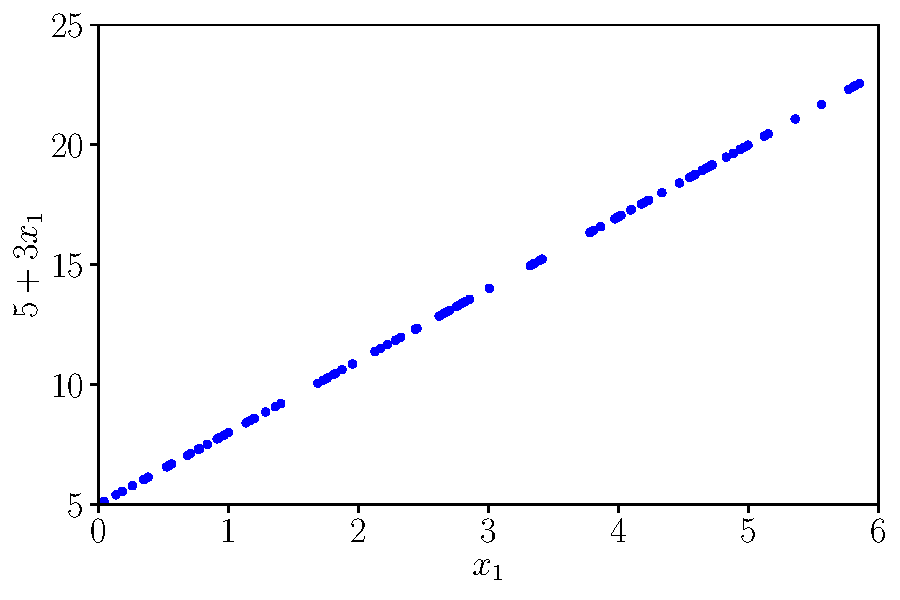
\includegraphics[width=0.6\textwidth]{einleitung/linear-data.pdf}
  \caption{Die generierte Daten}
  \label{plot:linear-data}
\end{figure}
\noindent
Die Daten sehen sehr gerade aus, damit das Problem nicht zu einfach
addieren auf Seiten der $y$ Werte zufälliges Rauschen.
\begin{lstlisting}
y += 3 * rng.standard_normal((100, 1))
\end{lstlisting}
Dies sollte das Problem ein wenig realistischer gestallten.
Die so modifizierten Daten sind in \autoref{plot:linear-data-noise} zu sehen.
\begin{figure}[h]
  \centering
  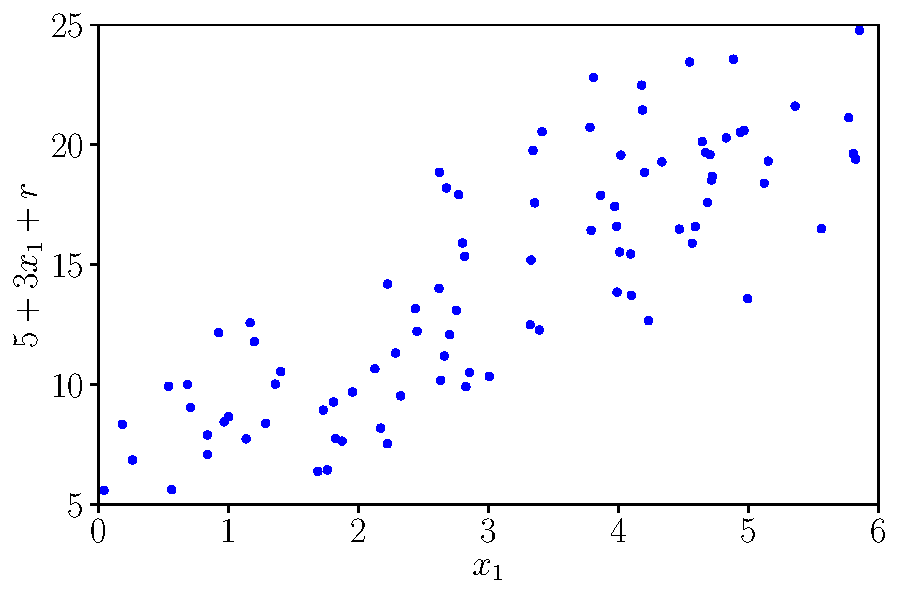
\includegraphics[width=0.6\textwidth]{einleitung/linear-data-noise.pdf}
  \caption{Die generierte Daten plus zufälliges Rauschen}
  \label{plot:linear-data-noise}
\end{figure}
Das Regressionsproblem besitzt eine Eingabe $x_1$ und eine Ausgabe $y$.
Ein echtes Problem besteht in der Regel aus mehreren Eingaben und manchmal
aus mehreren Ausgaben. Mehrdimensionale Daten lassen sich allerdings nur schwierig
visualisieren. Ziel des Modells ist es nun eine Gerade zu finden, welche die
Daten möglichst gut beschreibt. Die Geradengleichung hat die folgende Form:
\begin{align}
  \text{1 Feature}\qquad    & \yhat = \theta_0 + \theta_1 \cdot x_1   \\
  \text{$n$ Features}\qquad & \yhat = \theta_0 + \theta_1 \cdot x_1 +
  \theta_2 \cdot x_2 + \ldots + \theta_n \cdot x_n
\end{align}
Die griechischen Buchstaben Theta $\theta_i$ beschreiben die lernbaren Parameter und
der Funktionswert $\yhat$ (gesprochen \enquote{y-Hut}) beschreibt die Prognose.
Das Training kann in Python mit nur wenigen Zeilen Code durchgeführt werden:
\begin{lstlisting}
from sklearn.linear_model import LinearRegression
lin_reg = LinearRegression()
lin_reg.fit(x, y)
\end{lstlisting}
Wir verwenden das \lstinline{LinearRegression} Modell von Scikit-Learn
\footnote{\url{https://scikit-learn.org/stable/}} und rufen die \lstinline{fit}
Methode zusammen mit den Trainingsdaten und Labels auf, um das Modell zu trainieren.
Die trainierten Parameter befinden sich in den Attributen \lstinline{intercept_}
und \lstinline{coef_}:
\begin{lstlisting}
>>> lin_reg.intercept_, lin_reg.coef_
(array([4.84609918]), array([[3.03831479]]))
\end{lstlisting}
Nicht schlecht: Das Modell vermutet $\yhat = 4.85 + 3.04x_1$, wobei die ursprünglich
Funktion $y = 5 + 3x_1 + r$ war. Die genauen Werte konnten aufgrund des Rauschens
nicht gewonnen werden. Die Regressionsgerade zusammen mit den Daten ist
in \autoref{plot:linear-data-prediction} zu sehen.
\begin{figure}[!h]
  \centering
  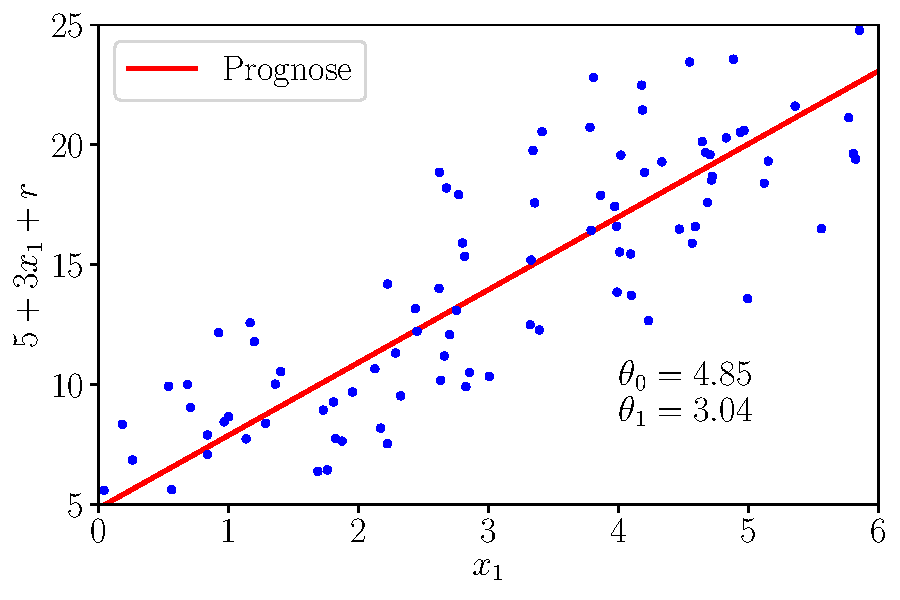
\includegraphics[width=0.6\textwidth]{einleitung/linear-data-prediction.pdf}
  \caption{Regressionsgerade}
  \label{plot:linear-data-prediction}
\end{figure}

\subsection{Unüberwachtes Lernen}